
\PassOptionsToPackage{svgnames}{xcolor}
\documentclass[10pt,letterpaper]{article}
\usepackage[top=.5in, bottom=.75in, left=.5in, right=.5in]{geometry}
\usepackage{tcolorbox}
\usepackage{lipsum}
\tcbuselibrary{skins,breakable}
\usetikzlibrary{shadings,shadows}

\usepackage{graphicx} % Allows to include images
\usepackage{booktabs} % Allows the use of \toprule, \midrule and \bottomrule in tables

\usepackage{multicol}
\usepackage{float}

\usepackage[T1]{fontenc}
\usepackage[utf8]{inputenc}

\title{\vspace{-.5in}Perfect Passing 2}
\author{\vspace{-.5in}}
\date{\vspace{-.5in}}

\newenvironment{agendablock}[1]{%
    \tcolorbox[beamer,%
    noparskip,breakable,
    colback=LightGray,colframe=Black,%
    colbacklower=Gray!75!LightGray,%
    title=#1]}%
    {\endtcolorbox}

\newenvironment{evenBlock}[1]{%
    \tcolorbox[beamer,%
    noparskip,breakable,
    colback=LightGreen,colframe=DarkGreen,%
    colbacklower=LimeGreen!75!LightGreen,%
    title=#1]}%
    {\endtcolorbox}

\newenvironment{oddBlock}[1]{%
    \tcolorbox[beamer,%
    noparskip,breakable,
    colback=LightBlue,colframe=DarkBlue,%
    colbacklower=DarkBlue!75!LightBlue,%
    title=#1]}%
    {\endtcolorbox}

\newenvironment{myexampleblock}[1]{%
    \tcolorbox[beamer,%
    noparskip,breakable,
    colback=LightGreen,colframe=DarkGreen,%
    colbacklower=LimeGreen!75!LightGreen,%
    title=#1]}%
    {\endtcolorbox}

\newenvironment{myalertblock}[1]{%
    \tcolorbox[beamer,%
    noparskip,breakable,
    colback=LightCoral,colframe=DarkRed,%
    colbacklower=Tomato!75!LightCoral,%
    title=#1]}%
    {\endtcolorbox}

\newenvironment{myblock}[1]{%
    \tcolorbox[beamer,%
    noparskip,breakable,
    colback=LightBlue,colframe=DarkBlue,%
    colbacklower=DarkBlue!75!LightBlue,%
    title=#1]}%
    {\endtcolorbox}

\usepackage{lmodern}

\begin{document}
\fontfamily{lmss}\selectfont


\maketitle

\section{Warm Ups}
\textbf{Time: 10 minutes}
\begin{agendablock}{Captain Led Warm ups / Coerver Touches (15 min) }
    \textbf{Warmups}
    \begin{enumerate}
        \item Jog to the 18 yard line and back twice with your ball (inside cut first time, outside cut the second),
        \item Side-Step to 18 yd line and back twice,
        \item Butt Kickers to the 18 yd line and back twice,
        \item Jog Backwards to the 18 yd line and back twice.
    \end{enumerate}
    \textbf{Touches}
    \begin{enumerate}
        \item Toe-Touches (20 count alternating feet).
        \item Pull back and Push Forward (10 each foot).
        \item Side to Side or Pendulums (20 count).
        \item Triangles (10 each foot).
        \item Pullback-Behind (20 count).
    \end{enumerate}
\end{agendablock}
\begin{evenBlock}{HOWTO:  Passing (5 min)}

\begin{minipage}[t]{\linewidth}
    \centering
    Review these elements prior to beginning the passing drills so its fresh in their heads.

    %\begin{minipage}{.3\linewidth} % Left column and width
        %\centering
        %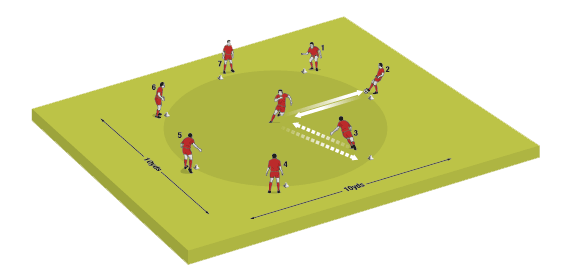
\includegraphics[width=\textwidth]{../img/Trimmed/Clocks1}
    %\end{minipage}
    %\hspace{0.05\linewidth}
    %\begin{minipage}{.6\linewidth} % Left column and width
    
        \textbf{Elements of the Pass:}
    
        \begin{enumerate}
        \setlength{\itemsep}{0pt}
        \setlength{\parskip}{0pt}
        \setlength{\parsep}{0pt}
        \item Ball should start about 1 step in front of the player.
        \item Non-kicking leg should be planted next to the ball with passer's toe pointed at the target.
        \item Ball should be struck in its center,
        \item With the inside portion of the foot.
        \item The kick should follow through.
        \end{enumerate}
        
        \textbf{Elements of the First Touch:}
        \begin{itemize}
        \setlength{\itemsep}{0pt}
        \setlength{\parskip}{0pt}
        \setlength{\parsep}{0pt}
        \item First before the ball is passed be sure you are ready, knees bent and on your toes.
        \item Move your body so the ball is coming directly to you.
        \item Bend your body over the ball as it comes in.
        \item Keep your eye on the ball as it comes into contact with your foot.
        \item Let your foot cushion the ball to slow it down and keep it near your feet.
        \item As your skill develops your first touch can move the ball into the space in which you want (open space or away from the defender).
        \end{itemize}

    %\end{minipage}
\end{minipage}

\end{evenBlock}

\clearpage

\section{Drills}

\textbf{Time: 5 minutes}
\begin{oddBlock}{Box Passing (10 min)}

\begin{minipage}[t]{\linewidth}
    \centering
    
    \begin{minipage}{.3\linewidth} % Left column and width
        \centering
        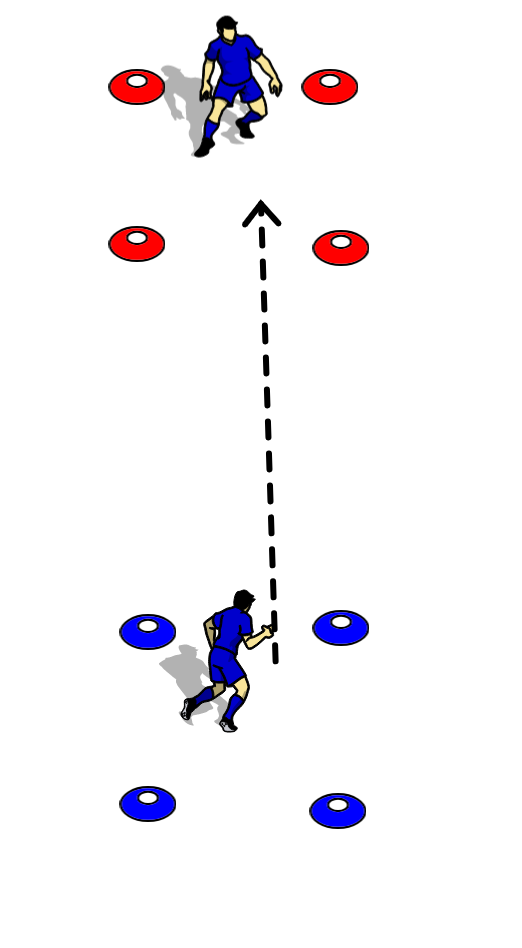
\includegraphics[width=.6\textwidth]{../img/Trimmed/Box_Passing_BW}
    \end{minipage}
    \hspace{0.05\linewidth}
    \begin{minipage}{.6\linewidth} % Left column and width
        \textbf{Drill Description:}

        \begin{enumerate}
        \setlength{\itemsep}{0pt}
        \setlength{\parskip}{0pt}
        \setlength{\parsep}{0pt}
        \item Two players stand in a 2 yard square box.  Boxes should be spaced about 5 yards apart.
        \item Players pass the ball to their partner in the 2 yard box.
        \item The partner tries to trap the ball within the box and pass it back.
        \item Alternate passing \& trapping foot half way through drill.
        \end{enumerate}

        \textbf{Coaching Points:}
        \begin{itemize}
        \setlength{\itemsep}{0pt}
        \setlength{\parskip}{0pt}
        \setlength{\parsep}{0pt}
        \item Focus on passing accurately with pace.
        \begin{itemize}
            \item Making a single step toward the ball.  This requires the ball to be one step in front of you.
            \item Hitting the center of the ball inside of your foot.
            \item Follow through.
        \end{itemize} 
        \item The goal is to trap the pass using a single touch.
        \item Stay on your toes at all times, this will keep you ready to move.  If you find it hard, focus on bouncing in place.
        \end{itemize}

    \end{minipage}
\end{minipage}

\end{oddBlock}

\textbf{Time: 5 minutes}
\begin{evenBlock}{Four Corner Passing}

\begin{minipage}[t]{\linewidth}
    \centering
    
    \begin{minipage}{.3\linewidth} % Left column and width
        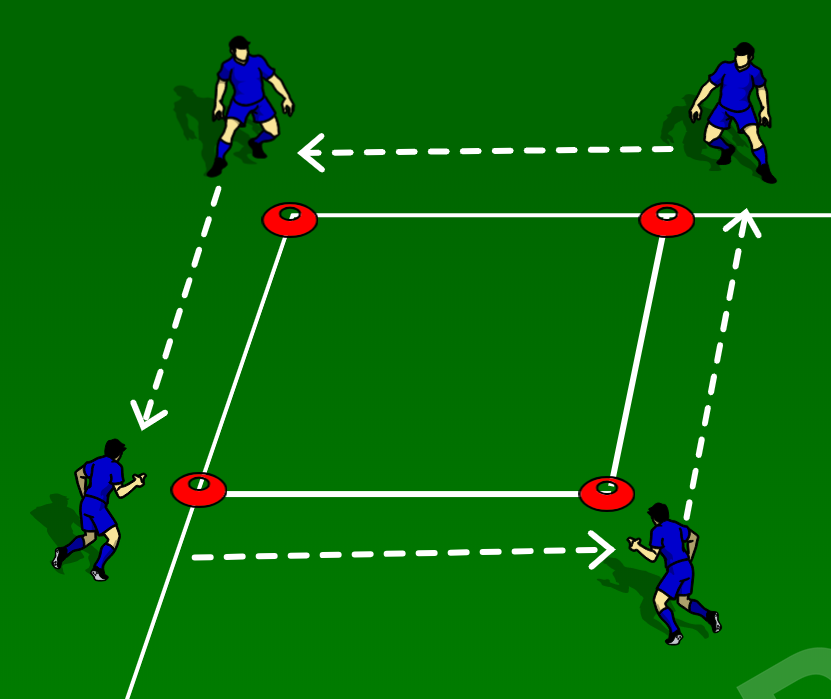
\includegraphics[width=.8\textwidth]{../img/Trimmed/Triangle_Passing_4P_mini}
    \end{minipage}
    \hspace{0.05\linewidth}
    \begin{minipage}{.6\linewidth} % Left column and width
        \textbf{Drill Description:}
        This drill focuses only on passing accurately and using the correct foot for the first touch.  This is like a 3 man passing drill around a box, but with an extra man so there is no movement element which should allow them to focus on the proper technique.
        \begin{enumerate}
            \setlength{\itemsep}{0pt}
            \setlength{\parskip}{0pt}
            \setlength{\parsep}{0pt}
            \item All players stand `open' to they can see all 3 of the players.
            \item The ball should be passed on one direction to start (to the left is more natural for a right footed player).
            \item The player receiving the ball should move his body so he receives the ball on his left foot then passes it to the next player using his right.
            \item After 5 rounds around the box, switch directions.  Pass to the right using the left foot, trap with the right.
        \end{enumerate}
    \end{minipage}

        \raggedright
        \textbf{Coaching Points:}
        \begin{itemize}
            \setlength{\itemsep}{0pt}
            \setlength{\parskip}{0pt}
            \setlength{\parsep}{0pt}
            \item Explain the first touch with the correct foot is the most important part.
            \item The touch should place the ball one step away from the player so they can step into and make a strong pass.
            \item The goal is to use two touches, not 1 and not 3.
            \item Once the passing and trapping with the correct foot becomes more natural, allow then to change directions at will, but any two adjacent players can't pass the ball back and forth more than 3 times.
        \end{itemize}

    
\end{minipage}

\end{evenBlock}

\textbf{Time: 10 minutes}
\begin{evenBlock}{Triangle Passing}
\textbf{Drill Description:}
        This drill is like the `4 Corner Passing Drill' but incorporates player movement to insure the player with the ball always has two options to pass too.
        If the groups are uneven, a `defender' can be added to the box.  If the pass goes through the box the passer switches location with the defender.  If trap is on the wrong foot the trapper switches with the defender.  Defenders count 5 successful passes and they switch with a player.
\begin{minipage}[t]{\linewidth}
    \begin{minipage}{.3\linewidth} % Left column and width
        \centering
        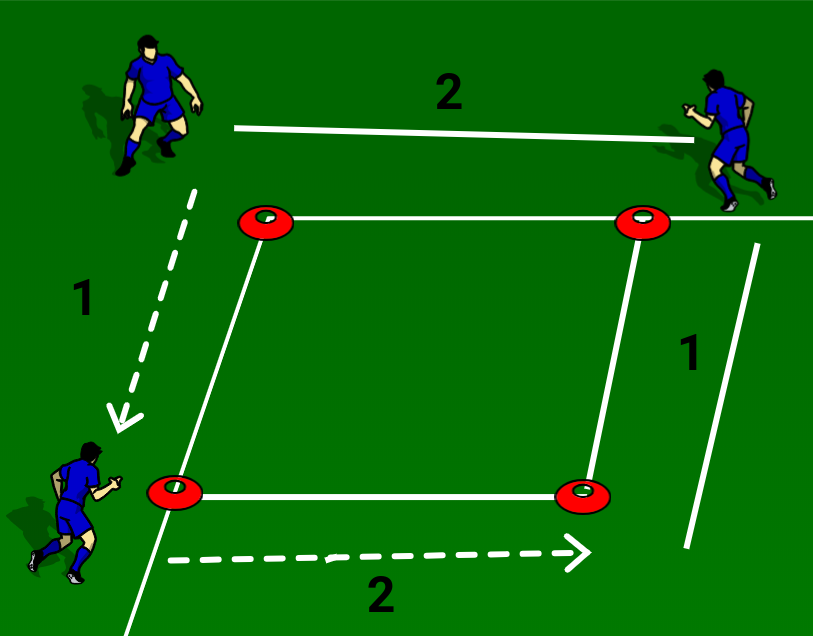
\includegraphics[width=\textwidth]{../img/Trimmed/Triangle_Passing_3P_mini}
    \end{minipage}
    \hspace{0.05\linewidth}
    \begin{minipage}{.6\linewidth} % Left column and width
        \begin{enumerate}
            \setlength{\itemsep}{0pt}
            \setlength{\parskip}{0pt}
            \setlength{\parsep}{0pt}
            \item All players stand `open' so they can see the other two players.
            \item The ball should be passed on one direction to start (to the left is more natural for a right footed player).
            \item The player receiving the ball should move his body so he receives the ball on his left foot then passes it to the next player using his right.  However the pass should wait until the 3 player is in position.
            \item  Player 3 (P3) was at a corner nearest the ball, however once the ball was passed, P3 needs to move to the other corner so they are again at a corner adjacent to the player with the ball.
            \item After 5 rounds around the box, switch directions.  Pass to the right using the left foot, trap with the right.
            \item After 5 additional rounds allow the player to switch directions at will, but any two adjacent players can't pass the ball back and forth more than 3 times.
        \end{enumerate}
    \end{minipage}
\end{minipage}
\raggedright
    \textbf{Coaching Points:}
    \begin{itemize}
        \setlength{\itemsep}{0pt}
        \setlength{\parskip}{0pt}
        \setlength{\parsep}{0pt}
        \item Explain the first touch with the correct foot is the most important part.
        \item The touch should place the ball one step away from the player so they can step into and make a strong pass.
        \item The goal is to use two touches, not 1 and not 3.
    \end{itemize}

\end{evenBlock}

%The following can be optional if time is running short.  Getting in the Small Sided activity and/or the Small Sided game should take precedence over the next drill at this practice.

%\textbf{Time: 8 minutes}
%\begin{evenBlock}{Figure 8 Passing (10 min)}

\begin{minipage}[t]{\linewidth}
    \centering
    
    \begin{minipage}{.3\linewidth} % Left column and width
        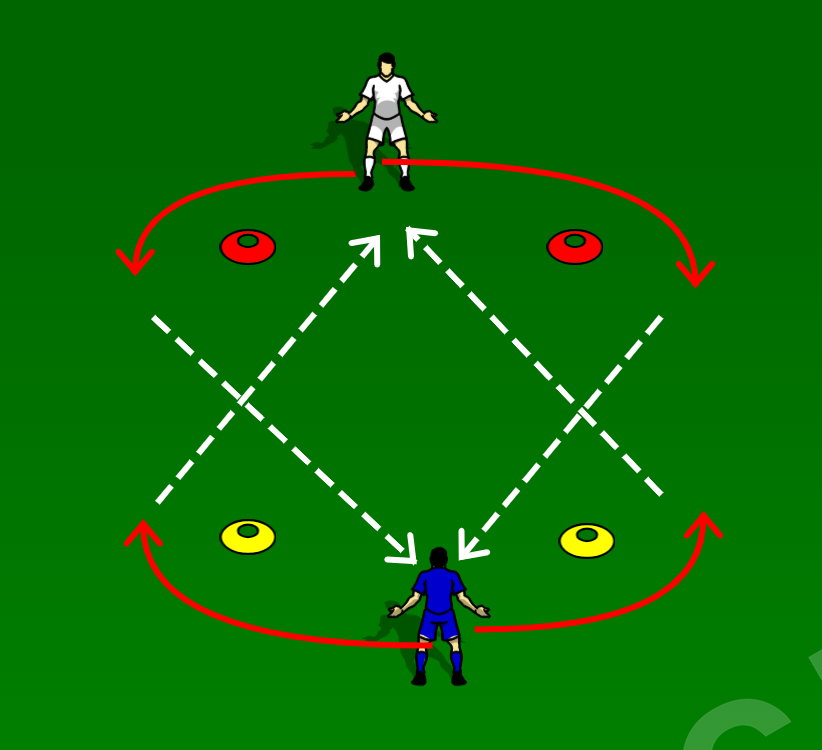
\includegraphics[width=\textwidth]{../img/Trimmed/Figure-8}
    \end{minipage}
    \hspace{0.05\linewidth}
    \begin{minipage}{.6\linewidth} % Left column and width
        \textbf{Drill Description:}
        This drill incorporates a lot of movement and passing.  Its designed to make the player trap and touch a ball around a defender for a clear pass.
        \begin{enumerate}
            \setlength{\itemsep}{0pt}
            \setlength{\parskip}{0pt}
            \setlength{\parsep}{0pt}
            \item Player 1 starts with the ball between two cones.  P2 starts between two cones the same width apart as P1 and 5 yards away.
            \item P1 dribbles around the cone on the right and passes to P2.
            \item P2 should trap the ball with the right foot and dribble around the right cone and pass to P1, who needs to race back between the two cones.
            \item This time P1 traps with the left foot and dribbles around the left cone and passes to P2.  P2 needs to race back between the two cones.
            \item P2 traps with the left and dribbles around the left cone to pass back to P1.
            \item At this point the drill repeats to the right side.
            \item After 10 passes stop and the P2 becomes the starting player.
        \end{enumerate}
    \end{minipage}
\end{minipage}

\textbf{Coaching Points:}
\begin{itemize}
    \setlength{\itemsep}{0pt}
    \setlength{\parskip}{0pt}
    \setlength{\parsep}{0pt}
    \item The cones are the defender, the goal is practice making that first touch and follow on touches into the open space then pass.
    \item Explain the first touch with the correct foot is important in guiding the ball into the open space.
    \item The goal would be able to use only 2 touches before making that third touch (the pass). 
    \item However I would rather see 3, 4 or 5 tight controlled touches than only 2 sloppy touches.

\end{itemize}


\end{evenBlock}


\textbf{Time: 10 minutes}
\begin{evenBlock}{Foot Soldiers (10 min)}

\begin{minipage}[t]{\linewidth}
    \centering
    
    \begin{minipage}{.4\linewidth} % Left column and width
        \centering
        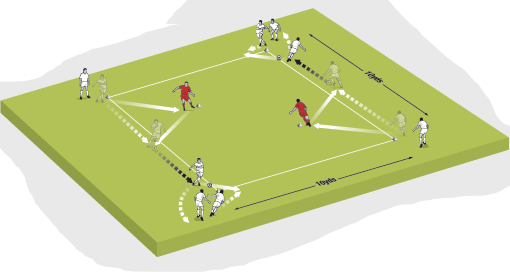
\includegraphics[width=\textwidth]{../img/Trimmed/FootSoldiers1}
        \vspace{6pt}
        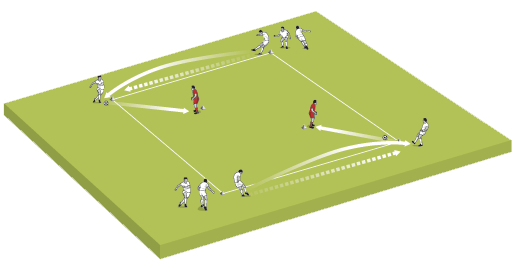
\includegraphics[width=\textwidth]{../img/Trimmed/Footsoldiers2}
    \end{minipage}
    \hspace{0.05\linewidth}
    \begin{minipage}{.5\linewidth} % Left column and width
        \textbf{Drill Description:}
        To use this simple warm-up mark out a 10x10-yard square with cones. Position a cone as shown for the central players. We have used 14 players in this activity, including two servers. You need balls and cones.
        \begin{enumerate}
        \setlength{\itemsep}{0pt}
        \setlength{\parskip}{0pt}
        \setlength{\parsep}{0pt}
        \item Place the two servers inside the square and arrange the remaining players around the four corners of the area use the central players to make one-two wall passes on opposite sides of the square and a first-time pass along the other sides of the square.
        \item Players should sidefoot their passes to the central players, who must make sure that they control the ball and pass it back to the running players so they don’t have to break their stride.
        \item You should swap the players over regularly, changing the two central wall passers. You must have two balls in play at once.
        \end{enumerate}

        \begin{enumerate}
        \setlength{\itemsep}{0pt}
        \setlength{\parskip}{0pt}
        \setlength{\parsep}{0pt}
        \item Play starts on both sides with a pass to the server who plays a one-two with the working player
        \item The player dribbles towards the cone and passes to the player at the cone
        \item The player at the next cone must be on the move to receive the ball and make a one touch pass to the next cone
        \item Players must follow the pass and keep moving around the square
        \item The receiving player for the one-two pass can take two touches because this needs to be an accurate move with a good weight on the pass
        \end{enumerate}

    \end{minipage}
\end{minipage}

\end{evenBlock}


\clearpage

\section{Small Sided Activity}
\textbf{Time: 15 minutes, Started at 1:15 PM to 1:20 PM}

\begin{evenBlock}{Clocks (10 min)}

\begin{minipage}[t]{\linewidth}
    \centering
    
    \begin{minipage}{.3\linewidth} % Left column and width
        \centering
        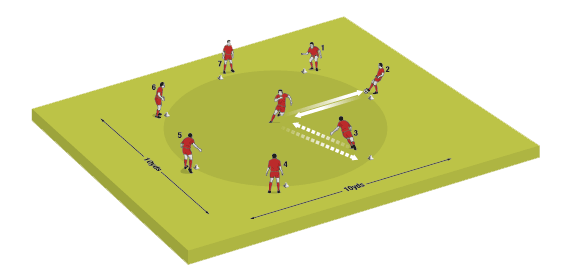
\includegraphics[width=\textwidth]{../img/Trimmed/Clocks1}
        \vspace{12pt}
        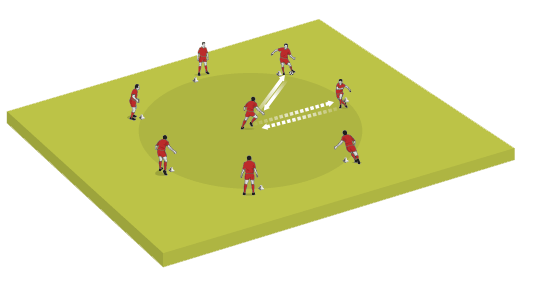
\includegraphics[width=\textwidth]{../img/Trimmed/Clocks2}
    \end{minipage}
    \hspace{0.05\linewidth}
    \begin{minipage}{.6\linewidth} % Left column and width
        \textbf{Drill Description:}
        Create a circle with your players of around 10 yards in diameter. Place cones around the circle where each player should stand, or go inside the centre circle and get the players to take a few steps forwards to get the right size. We’ve used eight players.
        \begin{enumerate}
        \setlength{\itemsep}{0pt}
        \setlength{\parskip}{0pt}
        \setlength{\parsep}{0pt}
        \item Start with the player in the middle who passes to one of the players around the circle
        \item Immediately the pass gets away, the centre player swaps position with the player clockwise from the player he passed to.
        \item The player he swaps with must get quickly into the centre to receive the ball and pass it to the next player anti-clockwise around the circle.
        \item Players continue to pass anti-clockwise and swap position with the player clockwise5. Try and get players to use one touch to get the ball around the clock
        \end{enumerate}
        
        \textbf{Coaching Points:}
        \begin{itemize}
        \setlength{\itemsep}{0pt}
        \setlength{\parskip}{0pt}
        \setlength{\parsep}{0pt}
        \item Focus on who gets your pass and then where you need to move.
        \item Attempt to complete this drill using a single touch.
        \end{itemize}

    \end{minipage}
\end{minipage}

\end{evenBlock}

\begin{evenBlock}{Press \& Protect}

\begin{minipage}[t]{\linewidth}
    \centering
    
    \begin{minipage}{.4\linewidth} % Left column and width
        \centering
        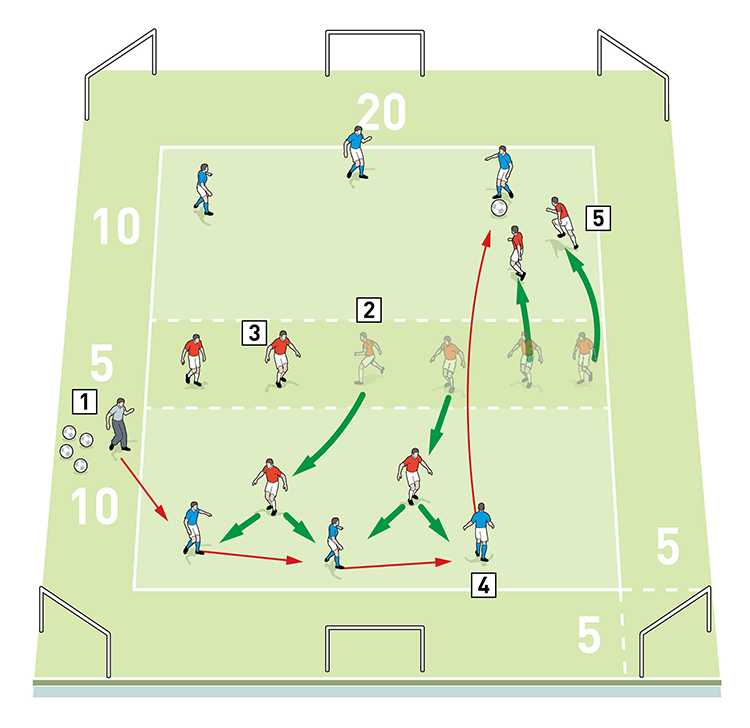
\includegraphics[width=\textwidth]{../img/Trimmed/Press_Protect}

        \vspace{6pt}
        
        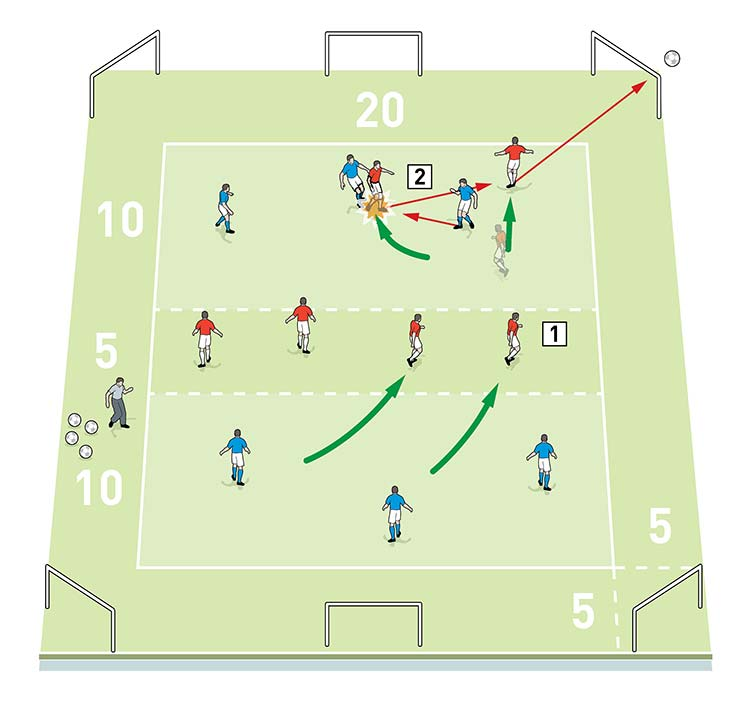
\includegraphics[width=\textwidth]{../img/Trimmed/Press_Protect_2}
    \end{minipage}
    \hspace{0.05\linewidth}
    \begin{minipage}{.5\linewidth} % Left column and width
        \textbf{Drill Description:}
        A drill that focuses on pressing and quick decision making for the passing team.  It also works on showing the importance of the center field player in their role of blocking through balls.
        
        \begin{enumerate}
        \setlength{\itemsep}{0pt}
        \setlength{\parskip}{0pt}
        \setlength{\parsep}{0pt}
        \item 20x25 yard area with a 5 yard middle zone.
        \item The pressing team of 6 stage in the middle, the other team (defending team) splits into 2 groups of 3 in on 10x20 side areas.
        \item 6 goals are positioned around 5 yard outside the area - the pressing team can score by passing the ball through any of these 6 goals.
        \item Coach is on the side line passing balls in.
        \item The pressing team is trying to score goals.
        \item The defending team is playing keep away and can pass to the other side.  At which point the press has to return to the center box 2 other players from the center box come out to press the other side.
        \item Switch roles every 5 minutes or 1/4 of the allocated time.
        \end{enumerate}

        \textbf{Coaching Points:}
        \begin{enumerate}
        \setlength{\itemsep}{0pt}
        \setlength{\parskip}{0pt}
        \setlength{\parsep}{0pt}
        \item Make quick passes.
        \item Think where should I pass the ball all the time (especially when the ball is not at your feet).
        \end{enumerate}
    \end{minipage}
\end{minipage}

\end{evenBlock}

\section{Game}

\textbf{Start Time: 1:35 PM}

\begin{oddBlock}{Small Sided}
    \textbf{Time:} 10 minute halves.

    \textbf{Size:} 4v4 or 5v5.

\end{oddBlock}

\section{Close}
\begin{oddBlock}{Sprints (5 min)}
\end{oddBlock}

\end{document}